\section{Study 2: Coordinate Banks and Original Characterization}
\label{app:characterization}

This appendix retains the original coordinate characterization,
which was specified after the excluded development comparisons.
It contains 72 model--readout--domain cells:
six models, four readouts, and three domains.
The 120 evaluation records comprise one C7 stratum, one D4
stratum, and three S3 strata in each of the 24 model/readout
conditions; they are not 120 independent random partitions.
The input-only field comparisons cover the 48 C7/D4 cells.
The results are descriptive aggregates of inspected outputs.
Original source flags and failed decisions remain in the archive,
and these outputs cannot serve as untouched data for later
method selection.
The later compact, transport, and spectral analyses retain
their separate evaluation contracts.

\paragraph{Data and information conditions.}
All six pinned base models use four readouts and training-only
$q=16$ PCA coordinates.
Model extraction uses BF16 and coordinate analysis uses float64.
The original execution added 41,728 extracted rows per model:
896 C7, 512 D4, and 40,320 S3 rows, including separately charged
support.
These are newly extracted rows in that execution, not the size
of the complete merged training, validation, and test banks.
For C7/D4, training and validation reuse the construction
caches, while the added rows form 64 test families with two
variants and complete state sets.
This original test construction is distinct from the later
64-family authored bank in \cref{sec:new-context}.

The S3 task permutes the assignments of three entities to
three roles, giving six abstract assignment states.
Its new-context, new-entity, and jointly new strata contain
$64\times24$, $48\times16$, and $64\times16$ family/entity
combinations, respectively.
Each combination has two variants and six states.
The resulting row counts are 18,432, 9,216, and 12,288;
384 additional support rows complete the total of 40,320.
The C7/D4 readout averages the state-token span.
S3 instead uses the final-token representation after the
complete role-assignment prompt.
New S3 entities therefore test transfer to held-out names
and triples while retaining the six abstract assignment states.
The C7/D4 state vocabulary is already seen in construction.
Holding out composite actions does not hold out those state
identities or create independently authored grammar roots.

Coordinate fields receive source coordinates and a requested
action, with supervised source--target training pairs.
The decoded-centroid benchmark additionally receives training
state labels and the exact action table, but decodes the
source state at evaluation.
The prediction contrasts in
\cref{tab:characterization-intervals} instead use
validation-selected oracle-source category/retention controls,
with an input-metadata potential also available for S3.
These are distinct information conditions.

\paragraph{Losses, fitting, and aggregation.}
The characterization normalizes squared errors by training-only
energy scales.
The Study~1 loss $D$ in \cref{eq:D} instead normalizes each row
by its target energy, so values across these studies are not
interchangeable.
Writing $\bar z_{\rm tr}$ for the training coordinate mean,
define
\[
 E_z=\mathbb E_{\rm tr}\|z-\bar z_{\rm tr}\|_2^2.
\]
For the two paraphrases of a family, ordered by their
registered identifiers, set
\[
 u_i=z_{p_0,i}-z_{p_1,i},
 \qquad E_u=\mathbb E_{\rm tr}\|u_i\|_2^2,
\]
without recentering the differences.
Coordinate prediction uses
$\|\widehat z_g-z_{g(i)}\|_2^2/E_z$.
The context endpoint fits a separate family of linear maps
$Q_g$ directly to training difference pairs $(u_i,u_{g(i)})$.
Its row-level contrast is
\[
 \Delta_{\rm ctx}(i,g)
 =
 \frac{\|\alpha u_i-u_{g(i)}\|_2^2
       -\|u_iQ_g-u_{g(i)}\|_2^2}{E_u},
\]
where the scalar-retention coefficient $\alpha$ is selected
separately on validation data.
Positive values favor the difference-fitted map.
The coordinate and difference fits each select one ridge
coefficient shared across actions within their condition.
Thus the original context contrast is difference fitting
versus scalar retention, not the later comparison of
difference fitting with coordinate fitting.

For prediction and context endpoints, validation and evaluation
retain changed-state pairs, $g(i)\ne i$.
All-element fitting uses all training pairs, including
identity and fixed-point pairs.
Generator-only fitting and selection use only the primitives.
The separate cycle and relation diagnostics have their own
complete-state evaluation rules.
Study~1's nonidentity-action prediction average retains D4
fixed-point pairs; the primary endpoints here exclude them.

Validation selection first averages changed-state errors
within each action and then gives actions equal weight.
The original reported prediction and context summaries
instead pool changed-state pairs within each family/entity
unit.
D4 actions move different numbers of corners, so these two
weightings need not agree.
The later compact endpoint uses equal-action evaluation
(\cref{app:aggregation-contract}).
Neither endpoint is the complete-bank, full-group,
second-moment-whitened class risk of
\cref{eq:class-loss-main}.

For resampling, the 24 fixed model/readout conditions are
first averaged within each family/entity unit.
The grids are $64\times1$ for C7/D4,
$64\times16$ for jointly new S3 contexts/entities,
$64\times24$ for new S3 contexts, and
$48\times16$ for new S3 entities.
The C7/D4 single column is a placeholder for family-only
resampling.
S3 independently resamples the family and entity indices.
The 10,000 percentile draws use seed 314159 and keep fitted
predictors and selected parameters fixed.
They do not repeat fitting or selection, sample a population
of models, or supply calibrated superiority, equivalence,
or multiplicity-controlled decisions.
\begin{table}[htbp]
\caption{Original characterization contrasts on the grammar-derived held-out banks, with recorded 95\% percentile sensitivity intervals (10,000 draws, seed 314159). Prediction compares validation-selected oracle-source category/retention controls, additionally including the S3 input-metadata potential, with coordinate Ridge. Context compares scalar retention with maps fitted directly to training paraphrase differences. Each contrast is baseline minus fitted-map loss, so positive values favor the fitted map. The endpoints use different training-energy denominators and pool changed-state pairs. Fitted models and selections remain fixed during family or crossed family/entity resampling. These banks and comparators differ from the later authored-context study.}
\label{tab:characterization-intervals}\centering\small
\begin{tabular}{llrrr}\toprule
Domain / split & Endpoint & Baseline minus linear & Lower & Upper \\
\midrule
$C_7$, new context & prediction & -0.002887 & -0.003290 & -0.002495 \\
$C_7$, new context & context & 0.011485 & 0.009997 & 0.013087 \\
$D_4$, new context & prediction & 0.019612 & 0.014730 & 0.025945 \\
$D_4$, new context & context & 0.060918 & 0.049883 & 0.072920 \\
$S_3$, context & prediction & -0.000487 & -0.000791 & -0.000249 \\
$S_3$, context & context & 0.000177 & 0.000010 & 0.000348 \\
$S_3$, entity & prediction & 0.000673 & 0.000443 & 0.000927 \\
$S_3$, entity & context & 0.000739 & 0.000542 & 0.000978 \\
$S_3$, joint & prediction & 0.000460 & 0.000262 & 0.000673 \\
$S_3$, joint & context & 0.000154 & -0.000017 & 0.000338 \\
\bottomrule\end{tabular}
\end{table}


\paragraph{Prediction and compact category controls.}
All-element direct Ridge and full-support kernel means are
$0.014900/0.004626$ for C7 and $0.041349/0.020916$ for D4.
Let $\mu_i$ be the training centroid for state $i$, and define
the nearest-centroid decoder and displacement predictor by
\[
 \widehat i(z)=\arg\min_{i\in S}\|z-\mu_i\|_2,
 \qquad
 \widehat z_g
 =z+\mu_{g(\widehat i(z))}-\mu_{\widehat i(z)}.
\]
Source decoding is perfect on the observed validation and
test input coordinates in all 48 C7/D4 field conditions.
The C7 mean error is $0.012013$, below Ridge's mean but
lower in only 9/24 conditions.
The D4 mean is $0.062349$, above Ridge's mean and lower
in only 2/24 conditions.
These original pooled endpoints differ from the later
compact comparison, including its D4 centroid/Ridge means
$0.063821/0.041919$ (\cref{app:aggregation-contract}).

The centroids store 112 and 64 floating-point coordinates
for C7 and D4, respectively, in addition to the integer
action table and decoding procedure.
This is a compact predictive control with explicit
construction labels, unlike fields that receive paired
targets but no explicit state labels.
Its accuracy does not establish native centroid decoding.
Applying a known composite label after one decode is also
different from repeatedly applying primitives and decoding
each intermediate output.
Perfect decoding of observed inputs does not certify that
repeated procedure.

\begin{figure}[t]
\centering
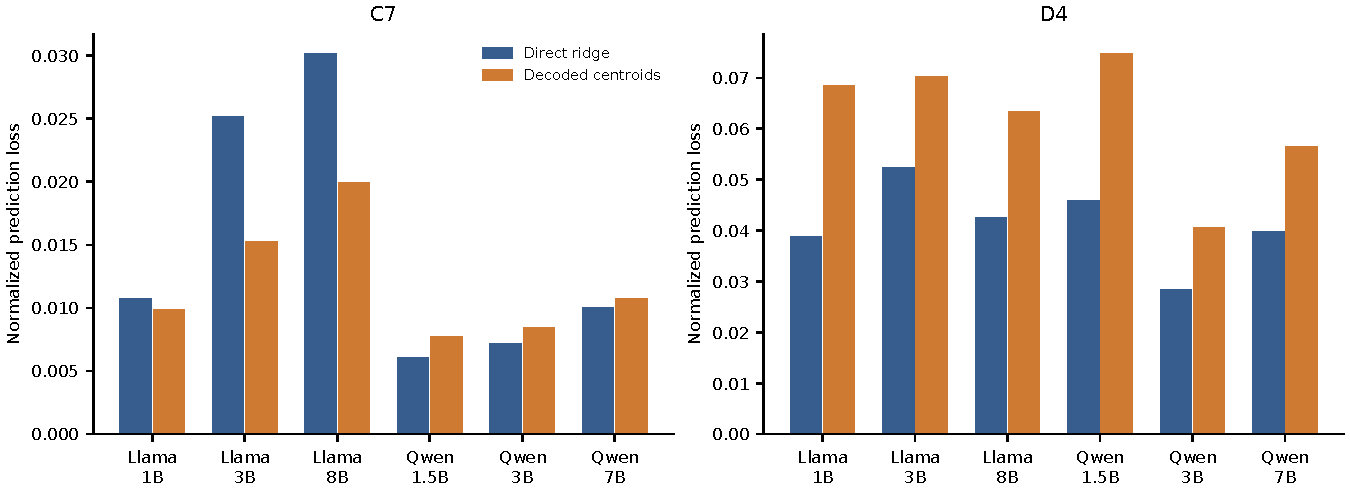
\includegraphics[width=.95\textwidth]
{figures/characterization_baselines.pdf}
\caption{
Original characterization prediction losses, pooling
changed-state pairs and averaging four fixed readouts
within each model.
C7 model means favor decoded centroids in the three
Llama models and Ridge in the three Qwen models;
D4 model means favor Ridge in all six.
These model means do not replace the condition-level
win counts and are not independent model-population draws.
The centroid predictor receives training labels and
the exact action table.
This is the original endpoint, not the later compact
comparison's equal-action aggregate.
}
\label{fig:characterization-baselines}
\end{figure}

\paragraph{Predictive accuracy and retained storage.}
The input-only field predicts a displacement by a normalized
Gaussian-weighted average of paired training displacements,
then adds it to the source coordinate.
Full support means retaining all training source points;
it does not mean using the full hidden dimension.
Primitive-only full fields store 21,504 versus 256 scalar
entries for C7 and 18,432 versus 512 for D4, relative to
the corresponding linear generator maps: factors of 84
and 36.
The small prescribed support budgets store 256 versus 256
for C7 and 480 versus 512 for D4.
The latter is near-budget rather than exactly matched.

On the original excluded-element prediction endpoint,
Ridge, full-support fields, and near-budget fields have
means $0.023176$, $0.004966$, and $0.700957$ for C7,
and $0.049005$, $0.023901$, and $0.212332$ for D4.
The lower full-support field errors therefore do not
establish an advantage at the small storage budgets.
Farthest-first support selection inspects all construction
source coordinates but retains only $K$ source points
and their paired displacements.
Linear regression instead compresses all construction
target pairs into its coefficients.
The original comparison did not train a compressed
nonlinear estimator on all target pairs.
The RFF/Nystr\"om extension in \cref{app:reproduction}
provides that separate comparison, with its own fitting,
identity handling, and aggregation.

All 48 full primitive fields select the smallest frozen
bandwidth multiplier, $0.125$; some reduced-support fits
select $0.25$.
These multipliers scale a training-source distance statistic,
rather than specify an absolute bandwidth.
Selection at the grid boundary limits what can be inferred
about the preferred scale.
A broader grid would require development-based specification,
not retrospective tuning on these test outcomes.

All-element Ridge stores a fitted identity-element matrix:
the recorded counts are 1792/2048 for C7/D4, or
1536/1792 when the identity is handled deterministically.
The $K=14$ fields store 1792/2016 entries, or 1568/1792
after removing zero identity-displacement arrays.
The pruned C7 field therefore retains 1,568 entries versus
1,536 for Ridge, about 2.1\% more.
The common PCA center and basis cost $d(q+1)$ float64
entries in this export.
Model weights, training memory, action tables, centroids,
biases, normalization, temporary arrays, and actual
precision must be accounted for where applicable.
Incremental stored-entry counts are neither total RAM
nor measures of statistical capacity.

\paragraph{S3 and context limitations.}
On the jointly new S3 context/entity stratum, identity
prediction loss is $0.018939$, compared with $0.018642$
for independent Ridge.
Here jointly new describes the evaluation stratum,
not the Joint estimator.
A small absolute loss alone is therefore weak evidence
of action recovery.
The corresponding context-contrast interval spans zero,
and the other S3 contrasts are small relative to the
original $0.01$ practical margin.
Neither observation establishes equivalence.
Support displacement gives prediction losses of
$0.015282$ on the joint stratum and $0.017580$ on new
entities, using four additional contexts per held-out
entity triple and assignment state.
These support observations are separately charged and
excluded from primary PCA and operator fitting;
the comparison is not zero-shot operator superiority.

The potential control is selected in the same 10/24
model/readout conditions across the three S3 strata,
yielding 30 stratum-specific records rather than
30 independent partitions.
Its neural optimization has not been independently
replayed.
The analytic difference fit is a separate estimator.
The original characterization adds no S3 coordinate-kernel,
native-intervention, or cross-model comparison.
Later context predictors and secondary extensions are
identified separately in \cref{app:reproduction}.

\paragraph{Relation to the later spectral diagnostics.}
The original predictive results above use their
training-derived coordinates and energy normalizations.
The spectral analysis instead characterizes complete
evaluated banks under its declared metric.
Within-template centering in
\cref{app:template-centering-sensitivity} operates only
in the saved 16-dimensional C7/D4 spaces and does not
recompute all predictors reported here.
The fixed-whitening treatment reports $C_{16}/16$
budgets and registration ranks; rewhitening additionally
changes the metric.
Neither procedure measures state-dependent variation
discarded outside the retained space.
Competitive category prediction and unstable registration
preference are compatible findings.
These later diagnostics do not revise the original S3
results or independently reproduce its neural optimizers.

\paragraph{Audit and provenance boundary.}
The historical audit verified the returned archive's
checksum and 490-member identity, source/configuration
pins, model/readout grid, metadata banks, exported geometry,
and 56 frozen intervals.
Independent NumPy implementations and additional analytic
replay reproduced the supported coordinate calculations
within their recorded numerical tolerances.
These are computational checks on the same observations,
not independent scientific replications.

A separate historical S3 reserved cross-block bank contains
9,216 rows per model.
Its row identities and fitting/scoring masks were checked.
It is distinct from the 9,216 newly extracted entity-test
rows, despite the equal counts.
Input-feature preprocessing can enumerate nontraining
source metadata while giving nontraining rows zero fitting
weight.
This discloses access to source metadata without fitting
held-out targets; it is not a claim that every preprocessing
operation uses training metadata alone.

Compact exports do not independently verify the original
model forwards or raw-to-PCA fitting.
For the S3 potential's compressed metadata features, they
also do not verify every omitted repeated embedding row.
This limitation is distinct from the Study~1 lexical
repeat checks in \cref{app:dimension-rank-audit}.
Independent retraining of the neural Joint and potential
estimators remains outside the recorded analytic replay.
Original archive/source hashes and derivative identities
preserve these verification boundaries.
